\section{Elephant Agent Runtime Architecture}
\label{sec:architecture}

The Elephant Agent runtime is organized around five cooperating memory layers:
Matriarch Core / Personal Model, Elephant State, Episode / Loop / Step Trail,
Contextual Recall, and Background Learning. Foreground response, explicit
Personal Model updates, background reflect, and operator-managed capabilities
all write through governed boundaries, and each durable update remains
traceable to runtime Steps and source Episodes.

\begin{figure}[t]
  \centering
  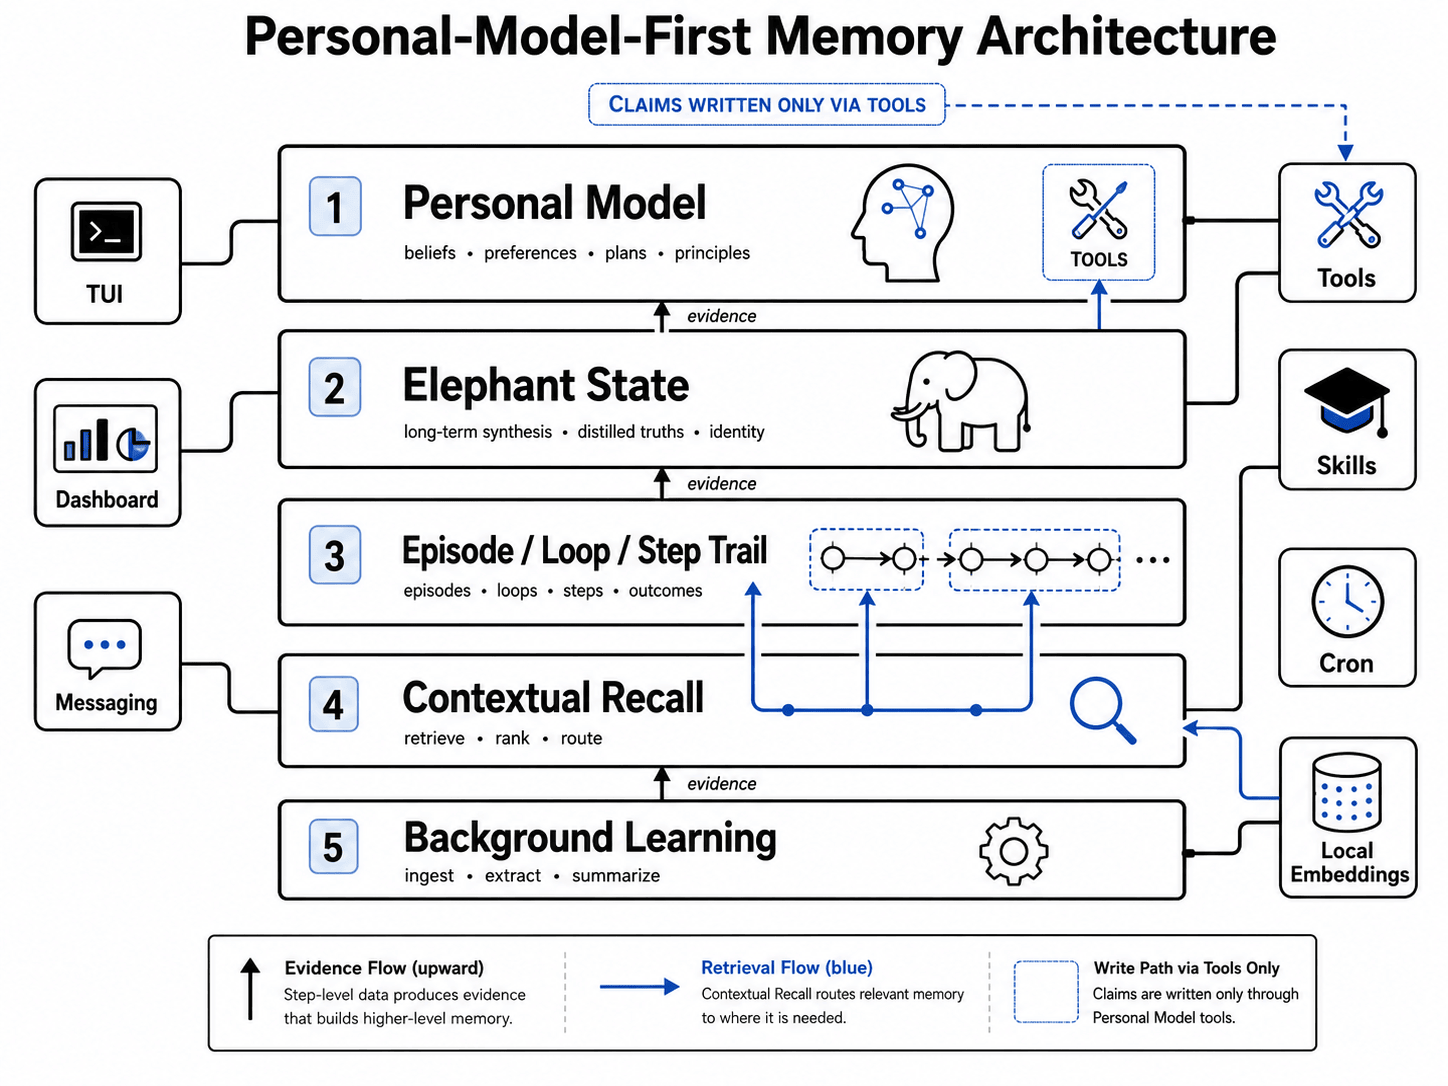
\includegraphics[width=\linewidth]{../../apps/site/static/assets/resources/paper-2.png}
  \caption{Elephant Agent's Personal-Model-first memory architecture. Evidence
  flows upward from Step-level source material; contextual recall retrieves
  support for the current turn; durable claims are written only through governed
  Personal Model tools.}
  \label{fig:runtime-architecture}
\end{figure}

\subsection{Runtime Planes}

The system is easier to reason about as five planes that cooperate at runtime.
The \textbf{surface plane} accepts triggers from the chat TUI, Dashboard,
messaging gateways, API calls, cron jobs, and background jobs. The
\textbf{response plane} owns the current foreground answer: it resolves the elephant,
selects provider and model posture, calls tools, and returns a response,
pause, or handoff. The \textbf{continuity plane} owns Elephant State, Episodes,
Loops, and Steps, so every answer has an execution trail. The
\textbf{understanding plane} owns Personal Model facts and open questions. The
\textbf{learning plane} owns background LearningJobs that read Step packets and
write back through Personal Model tools.

The important design decision is that these planes do not collapse into one
prompt. A wake prompt is a projection of state. It can include the elephant identity,
active facts, a compact Episode opening note, tool policy, and current-turn
recall support. The durable owners remain the tables and tools behind those
projections.

\subsection{Persistence Ownership}

The clean persistence model is organized around ownership boundaries, not a
single memory table:

\begin{center}
\begin{tabularx}{0.98\linewidth}{@{}lX@{}}
\toprule
\textbf{Table} & \textbf{Role} \\
\midrule
PersonalModel & One durable understanding container per user. \\
Facts & Active, retired, or disputed lens/topic claims. \\
OpenQuestions & Proactive curiosity prompts and their lifecycle. \\
State & Elephant identity plus one current context note. \\
Episode / Loop / Step & Runtime windows, interaction rounds, and atomic events. \\
SemanticIndexEntry & Vectorized Step or Fact chunks for contextual recall. \\
LearningJob & Background reflect task queue and result JSON. \\
\bottomrule
\end{tabularx}
\end{center}

Steps are the canonical conversation record. Facts carry source Episode
provenance.

\subsection{Foreground Response}

The foreground response loop is responsible for the current answer or
execution. It resolves the elephant, loads active Personal Model facts and relevant
State context, opens or reuses an Episode, starts a Loop, appends Steps, calls
tools, and produces a response or handoff.

Prompt text is a projection of governed runtime state. It may contain active
facts, an Episode opening resume snapshot, tool policy, and current-turn
\texttt{Current-turn recall support:} support. It is not the owner of those facts.

\subsection{Explicit Personal Model Update}

When the user explicitly asks Elephant Agent to remember, correct, forget, or dispute
something, the runtime treats that statement as foreground intent. The response
Loop calls \texttt{tool.personal\_model.update}. The update request names one
lens and topic, the proposed fact text when applicable, and the reason.

Low-risk, clear, user-directed captures may commit immediately. Ambiguous,
sensitive, identity-changing, cross-person, or high-impact captures require
stronger policy handling. Explicit Personal Model update is allowed in the
foreground because the user asked for it, but it still passes through typed
policy and can retire or dispute older facts.

\subsection{Claim-Aware Retrieval}

Current-turn recovery searches active facts. The search surface supports strict
exact lookup, conceptual semantic lookup, and verification. Exact mode disables
semantic drift and accepts only strict topic, phrase, token, or high-overlap
matches. Verify mode uses stricter
thresholds so weak similarity is not treated as belief. Semantic mode can use
translated or paraphrased query variants supplied by the model.

Every result is a claim-level answer with a status: strong match, weak match,
or no match. This status is part of the runtime contract. No match is a valid
answer when Elephant Agent lacks reliable Personal Model support.

\subsection{Background Reflect}

Inferred learning is handled outside the immediate reply. Background reflect is
a feature-composable agent system. A trigger selects features, the runner
builds an evidence packet from Episode Steps, the sub-agent uses foreground
tools such as \texttt{personal\_model.update} and
\texttt{personal\_model.questions}, and the runner persists its summary in
\texttt{learning\_jobs.result\_json}.

\begin{center}
\texttt{Trigger -> features -> Step packet -> reflect agent -> tools -> result\_json}
\end{center}

Supported trigger families include \texttt{episode\_close}, \texttt{manual},
\texttt{diary}, \texttt{dream}, \texttt{init\_profile}, and
\texttt{context\_compaction}. Reflect is part of Background Learning, not a
separate durable truth layer. It is a lifecycle that writes through existing
tools.

\subsection{Capability Path}

Tools, skills, models, cron jobs, messaging adapters, the chat TUI, and the
Dashboard make Elephant Agent operationally useful. They remain visible capabilities
around the Personal Model. When a workflow should become reusable, it remains
an explicit skill package or operator action. When the user corrects Elephant Agent, the
correction updates a Personal Model fact, not a hidden skill-affinity score.
